\documentclass[conference]{IEEEtran}
\IEEEoverridecommandlockouts
\usepackage{cite}
\usepackage{amsmath,amssymb,amsfonts}
\usepackage{graphicx}
\usepackage{textcomp}
\usepackage{xcolor}
\usepackage{booktabs}
\usepackage{array}
\usepackage{enumitem}
\usepackage{tikz}
\usetikzlibrary{arrows.meta,positioning}

\newcommand{\sat}{\operatorname{sat}}
\newcommand{\sign}{\operatorname{sign}}
\newcommand{\diag}{\operatorname{diag}}

\begin{document}

\title{Quanser QUBE-Servo 3 Rotary Pendulum:\\ Hardware Physics, Identification, Modelling, and the Complete Controller Suite\\
{\footnotesize Mathematical foundations for offline simulation, digital-twin, and hardware execution}}

\author{\IEEEauthorblockN{Gandhi Contreras}
\IEEEauthorblockA{\textit{Electrical and Computer Engineering}, New Mexico State University, Las Cruces, NM, USA \\ gandhico@nmsu.edu}}

\maketitle

\begin{abstract}
This paper develops the complete mathematical foundation of the Quanser QUBE-Servo~3 rotary inverted pendulum as an autonomous control platform. Unlike standard treatments that begin at the rigid-body equations, we expose the \emph{full physical chain}: the energy source, the PWM power amplifier, the brushed DC motor electromechanics, the mechanism and its friction physics, the quadrature encoders and tachometer, the acquisition and USB data path, and the real-time sampled-data loop --- every element that must be modelled for offline simulation, digital-twin, and hardware execution to agree. The rigid-body dynamics are derived by the Euler--Lagrange method and verified by Newton--Euler balances, yielding the nonlinear swing-up model and the linearized balance model, the two operating regimes that together constitute the full functionality of the robot. A grey-box identification methodology linear in the physical parameters is formulated, with one-step-ahead and free-run validation treated as distinct criteria. Finally, the complete controller suite is developed: PID with filtered derivatives, LQR, LQG, backstepping via collocated partial feedback linearization, sliding-mode control, energy-based swing-up with mode switching, and nonlinear model predictive control, including the implemented balance law and its safety envelope.
\end{abstract}

\begin{IEEEkeywords}
QUBE-Servo 3, Furuta pendulum, hardware physics, system identification, Euler--Lagrange, LQR, LQG, backstepping, sliding-mode control, NMPC, digital twin.
\end{IEEEkeywords}

%====================================================================
\section{Introduction}
The QUBE-Servo~3 is a rotary (Furuta) inverted pendulum: a DC motor drives a horizontal arm, and a pendulum rod pivots freely at the arm tip. Only the arm is actuated, so the system is underactuated with two mechanical degrees of freedom and one input. It exhibits the two canonical regimes of pendulum control: a \emph{global nonlinear regime} (swing-up, large $\alpha$) and a \emph{local unstable regime} (balance about the upright equilibrium). Mastery of both regimes, plus the mode logic that connects them, constitutes full functional use of the robot.

A model intended to serve three execution targets --- offline simulation, QLabs digital twin, and physical hardware --- must contain three layers that most papers omit or compress: (i) the \emph{power and actuation physics} from the supply to the shaft torque; (ii) the \emph{sensing and computation physics} from encoder optics to the sampled control loop; and (iii) the \emph{rigid-body mechanics}. Sections~\ref{sec:hw}--\ref{sec:sensors} develop layers (i)--(ii); Sections~\ref{sec:model}--\ref{sec:lin} develop layer (iii); Section~\ref{sec:id} gives the identification methodology; Section~\ref{sec:control} develops the controller suite. Throughout, $x=[\theta,\ \alpha,\ \dot\theta,\ \dot\alpha]^{\!\top}$, where $\theta$ is the arm angle about the vertical axis and $\alpha$ is the pendulum angle with $\alpha=0$ at the \emph{upright} position and $\alpha=\pi$ hanging down.

%====================================================================
\section{Hardware Physics: From the Energy Source to the Shaft}\label{sec:hw}

\begin{figure*}[!t]
\centering
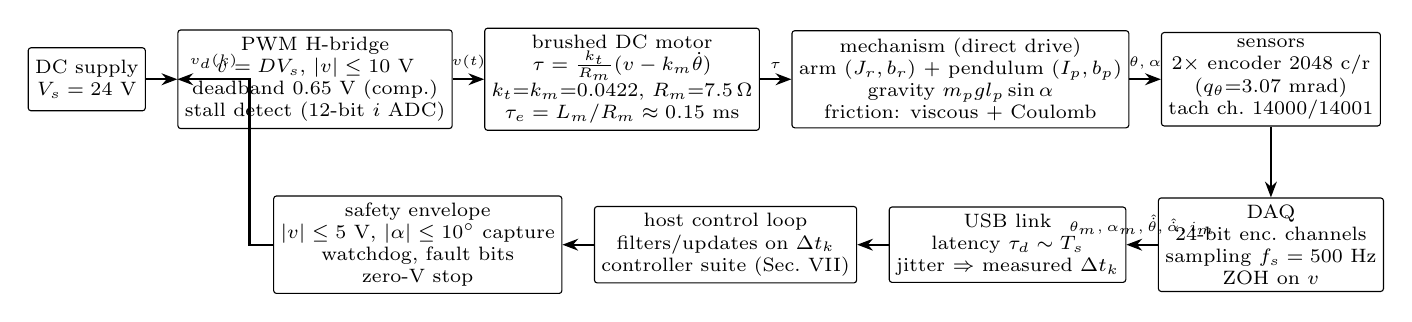
\begin{tikzpicture}[
  node distance=3mm and 4mm,
  blk/.style={draw, rounded corners=1pt, align=center, font=\scriptsize, inner sep=2.5pt, minimum height=8mm},
  lbl/.style={font=\tiny, align=center},
  arr/.style={-{Stealth[length=2mm]}, thick}
]
% forward power/actuation chain
\node[blk] (sup) {DC supply\\ $V_s = 24$ V};
\node[blk, right=of sup] (amp) {PWM H-bridge\\ $v = D V_s$, $|v|\le10$ V\\ deadband 0.65 V (comp.)\\ stall detect (12-bit $i$ ADC)};
\node[blk, right=of amp] (mot) {brushed DC motor\\ $\tau = \tfrac{k_t}{R_m}(v - k_m\dot\theta)$\\ $k_t{=}k_m{=}0.0422$, $R_m{=}7.5\,\Omega$\\ $\tau_e = L_m/R_m \approx 0.15$ ms};
\node[blk, right=of mot] (mech) {mechanism (direct drive)\\ arm $(J_r, b_r)$ + pendulum $(I_p, b_p)$\\ gravity $m_p g l_p\sin\alpha$\\ friction: viscous + Coulomb};
\node[blk, right=of mech] (enc) {sensors\\ $2{\times}$ encoder 2048 c/r\\ ($q_\theta{=}3.07$ mrad)\\ tach ch.\ 14000/14001};
% return sensing/compute chain
\node[blk, below=9mm of enc] (daq) {DAQ\\ 24-bit enc.\ channels\\ sampling $f_s = 500$ Hz\\ ZOH on $v$};
\node[blk, left=of daq] (usb) {USB link\\ latency $\tau_d \sim T_s$\\ jitter $\Rightarrow$ measured $\Delta t_k$};
\node[blk, left=of usb] (host) {host control loop\\ filters/updates on $\Delta t_k$\\ controller suite (Sec.\ VII)};
\node[blk, left=of host] (safe) {safety envelope\\ $|v|\le5$ V, $|\alpha|\le10^\circ$ capture\\ watchdog, fault bits\\ zero-V stop};
\draw[arr] (sup) -- (amp);
\draw[arr] (amp) -- node[lbl, above] {$v(t)$} (mot);
\draw[arr] (mot) -- node[lbl, above] {$\tau$} (mech);
\draw[arr] (mech) -- node[lbl, above] {$\theta,\alpha$} (enc);
\draw[arr] (enc) -- (daq);
\draw[arr] (daq) -- node[lbl, above] {$\theta_m,\alpha_m,\hat{\dot\theta},\hat{\dot\alpha},i_m$} (usb);
\draw[arr] (usb) -- (host);
\draw[arr] (host) -- (safe);
\draw[arr] (safe.west) -- ++(-3mm,0) |- node[lbl, pos=0.75, above] {$v_d(k)$} (amp.west);
\end{tikzpicture}
\caption{QUBE-Servo 3 signal chain with the physics carried by each stage (values verified against the user manual, Table~\ref{tab:params}). The loop closes through the safety envelope; every discrete update advances on the measured period $\Delta t_k$.}
\label{fig:chain}
\end{figure*}

\subsection{Power path}
The device is powered by a regulated external DC supply of voltage $V_s$ (per the QUBE-Servo~3 user manual), while the USB-C link carries only data and logic power. The supply feeds (a) the logic/DAQ electronics through low-dropout regulation and (b) the motor power stage. Two physical consequences matter for control: the achievable motor voltage is bounded by the supply and the amplifier headroom, $|v|\le V_{\max}$, and supply-rail droop under transient current couples all electrical subsystems, which is why aggressive commands are rate- and magnitude-limited in software.

\subsection{PWM power amplifier}
The motor is driven by an H-bridge operated by pulse-width modulation at a switching frequency $f_{\mathrm{pwm}}$ far above both the electrical pole of the motor and the control rate. Averaging over one switching period, the applied terminal voltage is
\begin{equation}
v(t) \;=\; D(t)\,V_s,\qquad D\in[-1,1],
\end{equation}
with duty ratio $D$ set by the command channel (the integrated DAQ emulates a linear amplifier on its analog-output channel; a raw PWM duty channel is alternatively exposed). The average model is exact for control purposes because $f_{\mathrm{pwm}}\gg 1/T_s$; the residual effects are a small ripple current of peak-to-peak amplitude $\Delta i \approx V_s/(4 L_a f_{\mathrm{pwm}})$ and a dead-time/deadband distortion near zero crossing --- on this unit a documented \emph{default deadband of $0.65$~V that the DAQ compensates in firmware} (the compensation is configurable and can be disabled, in which case the dead-zone re-enters the plant model). The recommended output range is $\pm10$~V ($\pm15$~V absolute) from the $24$~V supply. The amplifier is protected by \emph{stall detection}: the 12-bit current-sense ADC monitors the armature current (peak $1.8$~A at $15$~V, continuous $0.58$~A at $5$~V), and a prolonged stall with more than $5$~V applied disables the bridge; the digital I/O exposes stall-warning, stall-error, and amplifier-fault bits that the control software must poll (Section~\ref{sec:safety}).

\subsection{Brushed DC motor electromechanics}
The armature circuit obeys Kirchhoff's voltage law,
\begin{equation}
L_a \frac{di}{dt} + R_m\, i + e_b = v, \qquad e_b = k_m\,\dot\theta,
\label{eq:armature}
\end{equation}
where $e_b$ is the back electromotive force generated by the rotor flux linkage, and the electromagnetic torque is
\begin{equation}
\tau_m = k_t\, i .
\end{equation}
In SI units $k_t\,[\mathrm{N\,m/A}]$ and $k_m\,[\mathrm{V\,s/rad}]$ are numerically equal by energy conservation of the ideal transducer (verified on this unit: $k_t = k_m = 0.0422$). The electrical time constant $\tau_e = L_m/R_m = 1.15\,\mathrm{mH}/7.5\,\Omega \approx 0.15\,$ms, more than an order of magnitude below the $2$~ms sampling period, so \eqref{eq:armature} is quasi-static at the control rate:
\begin{equation}
\boxed{\;\tau = \frac{k_t}{R_m}\bigl(v - k_m\,\dot\theta\bigr)\;}
\label{eq:motor_static}
\end{equation}
The QUBE arm is \emph{direct drive} (no gearbox), so \eqref{eq:motor_static} is the shaft torque; there is no backlash and no gear efficiency factor. Two physical limits accompany \eqref{eq:motor_static}: the continuous thermal limit set by Joule heating $P_J = R_m i^2$ (the winding temperature obeys a first-order thermal model $C_{\mathrm{th}}\dot T_w = R_m i^2 - (T_w-T_a)/R_{\mathrm{th}}$), and the peak-current/demagnetization limit enforced by the amplifier current clamp.

Equation \eqref{eq:motor_static} has a structural consequence used throughout this paper: back-EMF acts as \emph{electrical damping}. Substituting \eqref{eq:motor_static} into the mechanics adds the term $-(k_t k_m/R_m)\dot\theta$, so the effective arm damping is
\begin{equation}
\bar b_r \;=\; b_r + \frac{k_t k_m}{R_m},
\qquad
k_v \;=\; \frac{k_t}{R_m},
\label{eq:emf_damping}
\end{equation}
and the voltage-level input gain is $k_v$. Identification (Section~\ref{sec:id}) estimates $\bar b_r$ and $k_v$ directly; separating $b_r$ from the electrical part requires a current measurement.

\subsection{Mechanism and friction physics}
The mechanism is two rigid links: the arm (length $L_r$ to the pendulum pivot) rotating about the vertical, and the pendulum rod (length $L_p$, centre of mass at $l_p$) rotating about the horizontal pivot fixed in the arm tip. Both joints run on ball bearings whose losses are captured by
\begin{equation}
\tau_f(\dot q) \;=\; b\,\dot q \;+\; \tau_c \tanh\!\Bigl(\frac{\dot q}{\epsilon}\Bigr)
\;+\;\bigl(\tau_s-\tau_c\bigr)\,e^{-(\dot q/v_s)^2}\sign(\dot q),
\label{eq:friction}
\end{equation}
i.e., viscous, Coulomb (smoothed with slope parameter $\epsilon$), and Stribeck terms; the Stribeck contribution matters near velocity reversals of the swing. In the nominal model only $(b_r, b_p)$ are retained, with \eqref{eq:friction} available as the refinement layer once identified.

%====================================================================
\section{Sensor and Computation Physics}\label{sec:sensors}

\subsection{Quadrature optical encoders}
Both angles are measured by incremental optical encoders: an LED--photodiode pair reads a slotted code wheel producing two square waves in quadrature ($90^\circ$ phase), decoded at $4\times$ to $N_{\mathrm{enc}}$ counts per revolution ($N_{\mathrm{enc}}=2048$ nominal per the user manual). The measurement model is exact quantization,
\begin{equation}
\theta_m = \frac{2\pi}{N_{\mathrm{enc}}}\,\Bigl\lfloor \frac{N_{\mathrm{enc}}}{2\pi}\,\theta \Bigr\rceil,
\qquad
q_\theta = \frac{2\pi}{N_{\mathrm{enc}}} \approx 3.07\,\mathrm{mrad},
\label{eq:quant}
\end{equation}
and identically for $\alpha$. Incremental encoders measure \emph{relative} angle: the count is zeroed at initialization, so the software must establish the reference (pendulum hanging at rest defines $\alpha_m = \pi$ after the offset convention is applied).

The central sensing problem is velocity. A finite difference of \eqref{eq:quant} has quantization-induced noise of standard deviation
\begin{equation}
\sigma_{\hat{\dot\theta}} \;\approx\; \frac{q_\theta}{T_s\sqrt{6}},
\end{equation}
which at $T_s=2\,$ms is of order $0.6\,$rad/s --- unusable for derivative feedback. Two remedies are modelled in this work: (i) the QUBE-Servo~3 DAQ provides \emph{digital tachometers} for both encoders (angular speed in counts/s on channels 14000/14001, i.e., hardware-timed edge-rate measurement, far smoother than a software finite difference), and (ii) a second-order filtered derivative is used on encoder angles,
\begin{equation}
\frac{\hat{\dot q}(s)}{q_m(s)} = \frac{\omega_f^2\, s}{s^2 + 2\zeta_f\omega_f s + \omega_f^2},
\label{eq:filtder}
\end{equation}
discretized with the \emph{measured} loop period each step (Section~\ref{sec:rt}). The filter adds phase lag $\angle \approx -2\zeta_f\omega/\omega_f$ at low frequency, a destabilizing effect that must be included in any stability analysis of derivative feedback.

\subsection{Current sensing}
The amplifier exposes the motor current through a shunt/monitor channel. Physically this measures the armature current of \eqref{eq:armature}; it enables torque estimation $\hat\tau = k_t i_m$, separation of $b_r$ from the back-EMF damping in \eqref{eq:emf_damping}, and detection of stall/overload.

\subsection{Acquisition, USB path, and the real-time loop}\label{sec:rt}
The DAQ samples all channels at the loop rate $f_s$ (500~Hz default in the vendor interface, $T_s = 2$~ms), applies zero-order hold to the output,
\begin{equation}
v(t) = v_d(k), \qquad t\in[kT_s,\,(k{+}1)T_s),
\end{equation}
and exchanges packets with the host over USB. The host operating system is not hard real time: the realized loop period $\Delta t_k$ is a random variable with mean near $T_s$ and occasional multi-millisecond excursions. The discipline adopted throughout this project --- and the single most important implementation lesson of our hardware campaigns --- is that \emph{all discrete-time integrations and derivative filters advance with the measured $\Delta t_k$, never the nominal $T_s$}:
\begin{equation}
\hat{\dot q}_{k} = \mathcal{F}\bigl(q_{m,k};\,\Delta t_k\bigr),\qquad \Delta t_k = t_k - t_{k-1}.
\label{eq:measured_dt}
\end{equation}
Latency enters as a one-to-two sample input delay $v(t-\tau_d)$, $\tau_d\!\approx\!T_s$, which subtracts phase $\omega\tau_d$ at the crossover frequency and therefore bounds the achievable bandwidth of any controller in Section~\ref{sec:control}.

\subsection{Safety envelope}\label{sec:safety}
For autonomous operation the following constraints are part of the plant definition, not afterthoughts:
\begin{enumerate}[label=\arabic*)]
\item actuation bound $|v| \le V_{\max}$; the implemented balance law uses the tighter operational bound $|v|\le 5$~V;
\item capture logic: full-authority balance feedback is enabled only inside $|\alpha| \le \alpha_c$ with $\alpha_c = 10^\circ$ (implemented value), preventing large torques from being commanded far from the linearization domain;
\item amplifier-fault monitoring (thermal shutdown) with commanded zero voltage on fault;
\item watchdog on stale measurements ($\Delta t_k$ above threshold $\Rightarrow$ zero command);
\item arm travel limits to protect the cable and workspace, $|\theta|\le\theta_{\max}$;
\item on any stop event: zero voltage, disable amplifier, log state.
\end{enumerate}

%====================================================================
\section{Nonlinear Modelling}\label{sec:model}

\subsection{Coordinates, kinematics, and energies}
Generalized coordinates $q = [\theta,\ \alpha]^{\!\top}$. With inertial frame $\{x,y,z\}$, $z$ up, define the arm-fixed radial/tangential unit vectors $e_r = [\cos\theta,\ \sin\theta,\ 0]^{\!\top}$, $e_t = [-\sin\theta,\ \cos\theta,\ 0]^{\!\top}$. The pendulum direction (from pivot toward the bob, upright at $\alpha=0$) is
\begin{equation}
u = \sin\alpha\, e_t + \cos\alpha\, e_z ,
\end{equation}
so the centre of mass sits at $r_c = L_r e_r + l_p u$ and its squared speed evaluates to
\begin{equation}
\|\dot r_c\|^2 = L_r^2\dot\theta^2 + l_p^2\dot\alpha^2 + l_p^2\sin^2\!\alpha\,\dot\theta^2 + 2L_r l_p\cos\alpha\,\dot\theta\dot\alpha .
\end{equation}
Define the composite parameters
\begin{equation}
J_a = J_r + m_p L_r^2,\qquad
I_p = J_p + m_p l_p^2,\qquad
h = m_p L_r l_p,
\label{eq:composite}
\end{equation}
where $J_r$ is the arm-side inertia about the vertical axis (motor rotor + hub + arm) and $J_p$ the pendulum inertia about its own centre of mass. The kinetic and potential energies are
\begin{align}
T &= \tfrac12\bigl(J_a + I_p\sin^2\!\alpha\bigr)\dot\theta^2 + h\cos\alpha\,\dot\theta\dot\alpha + \tfrac12 I_p\dot\alpha^2, \label{eq:T}\\
V &= m_p g l_p \cos\alpha .\label{eq:V}
\end{align}

\subsection{Euler--Lagrange equations}
With $\mathcal L = T - V$ and generalized forces $Q = [\tau - b_r\dot\theta,\ -b_p\dot\alpha]^{\!\top}$, $\frac{d}{dt}\partial_{\dot q_i}\mathcal L - \partial_{q_i}\mathcal L = Q_i$ yields the full nonlinear model
\begin{align}
&\bigl(J_a + I_p\sin^2\!\alpha\bigr)\ddot\theta + h\cos\alpha\,\ddot\alpha
+ I_p\sin(2\alpha)\,\dot\theta\dot\alpha \nonumber\\
&\qquad\qquad - h\sin\alpha\,\dot\alpha^2 + b_r\dot\theta = \tau,
\label{eq:nl1}\\[2pt]
&h\cos\alpha\,\ddot\theta + I_p\ddot\alpha - \tfrac12 I_p\sin(2\alpha)\,\dot\theta^2 \nonumber\\
&\qquad\qquad - m_p g l_p\sin\alpha + b_p\dot\alpha = 0 .
\label{eq:nl2}
\end{align}
Every term has a physical reading: $I_p\sin(2\alpha)\dot\theta\dot\alpha$ is the inertia modulation of the arm axis by the swinging pendulum; $h\sin\alpha\,\dot\alpha^2$ is the centrifugal reaction of the bob on the arm; $\tfrac12 I_p \sin(2\alpha)\dot\theta^2$ is the centrifugal torque that pushes the pendulum away from the vertical plane of rotation; $m_p g l_p \sin\alpha$ is gravity, destabilizing about $\alpha=0$.

\subsection{Manipulator form and structural properties}
Equations \eqref{eq:nl1}--\eqref{eq:nl2} are compactly
\begin{equation}
M(q)\ddot q + C(q,\dot q)\dot q + G(q) + F\dot q = B_u\,\tau,
\label{eq:manip}
\end{equation}
\begin{equation}
M = \begin{bmatrix} J_a + I_p \sin^2\!\alpha & h\cos\alpha\\ h\cos\alpha & I_p \end{bmatrix},\quad
B_u = \begin{bmatrix}1\\0\end{bmatrix},
\end{equation}
\begin{equation}
G = \begin{bmatrix}0\\ -m_p g l_p\sin\alpha\end{bmatrix},\quad
F = \diag(b_r,\,b_p),
\end{equation}
with $C(q,\dot q)$ the Coriolis/centrifugal matrix obtained from the Christoffel symbols of $M$. Three properties used by the controllers: $M = M^{\!\top}\!\succ 0$ (since $J_a I_p - h^2\cos^2\!\alpha + J_a I_p \sin^2\!\alpha > 0$ whenever $J_a I_p > h^2$, true for physical parameters); $\dot M - 2C$ is skew-symmetric (passivity); and the system is \emph{underactuated} with relative degree structure that forbids exact input--state linearization but admits the collocated partial feedback linearization used in Section~\ref{sec:bs}.

\subsection{Newton--Euler verification}
The same equations follow from momentum balances: for the pendulum, $m_p\ddot r_c = F_J + m_p g\,(-e_z)$ and $\dot H_c = M_J + (l_p u)\times F_J$ about its centre of mass, where $(F_J, M_J)$ are the joint reaction force and moment; for the arm, the axial moment balance about $e_z$ collects the motor torque, friction, and the reaction $-F_J$ acting at $L_r e_r$. Projecting the pendulum moment balance on its hinge axis $(-e_r)$ and the arm balance on $e_z$ reproduces \eqref{eq:nl1}--\eqref{eq:nl2} exactly; this derivation exposes the joint reaction $F_J$ explicitly, which is what a mechanical safety analysis (bearing load rating) consumes.

\subsection{Voltage-level model}
Substituting the actuator physics \eqref{eq:motor_static} and \eqref{eq:emf_damping} into \eqref{eq:manip} gives the model in the physically commanded input $v$:
\begin{equation}
M(q)\ddot q + C(q,\dot q)\dot q + G(q) + \bar F\dot q = B_u\,k_v\,v,
\quad \bar F = \diag(\bar b_r, b_p),
\label{eq:voltage_model}
\end{equation}
with $|v|\le V_{\max}$. Equation \eqref{eq:voltage_model} is the plant used by every controller in Section~\ref{sec:control} and by the digital twin.

\subsection{Equilibria and the two applications}
Setting derivatives to zero in \eqref{eq:voltage_model}: the \emph{hanging} equilibrium $\alpha = \pi$ (stable) and the \emph{upright} equilibrium $\alpha = 0$ (unstable), both with arbitrary $\theta$. These generate the robot's two applications:
\begin{enumerate}[label=(\alph*)]
\item \textbf{Swing-up} --- a global maneuver on the full nonlinear model \eqref{eq:voltage_model}, treated by energy control (Section~\ref{sec:swing});
\item \textbf{Balance} --- local stabilization of $\alpha=0$ with arm positioning, treated on the linearization (Sections~\ref{sec:lin}, \ref{sec:control}).
\end{enumerate}

\subsection{Pendulum energy}
For swing-up, define the pendulum-only energy referenced to the upright rest state,
\begin{equation}
E(\alpha,\dot\alpha) = \tfrac12 I_p\dot\alpha^2 + m_p g l_p\bigl(\cos\alpha - 1\bigr),
\label{eq:energy}
\end{equation}
so $E = 0$ at $(\alpha,\dot\alpha)=(0,0)$ and $E = -2m_p g l_p$ hanging at rest. Along trajectories of \eqref{eq:nl2} with the arm acceleration acting as the input,
\begin{equation}
\dot E = -\,h\cos\alpha\,\dot\alpha\,\ddot\theta \;-\; b_p\dot\alpha^2 ,
\label{eq:Edot}
\end{equation}
which shows that arm acceleration pumps or removes pendulum energy with sign $-\sign(\dot\alpha\cos\alpha)$ --- the mechanism exploited by the swing-up law.

%====================================================================
\section{Linearized Models}\label{sec:lin}

\subsection{Upright (balance) model}
Linearizing \eqref{eq:voltage_model} about $(\alpha,\dot\theta,\dot\alpha)=(0,0,0)$ with $\sin\alpha\!\approx\!\alpha$, $\cos\alpha\!\approx\!1$:
\begin{align}
J_a\ddot\theta + h\ddot\alpha + \bar b_r\dot\theta &= k_v v, \label{eq:lin1}\\
h\ddot\theta + I_p\ddot\alpha + b_p\dot\alpha - m_p g l_p\,\alpha &= 0. \label{eq:lin2}
\end{align}
With $\Delta = J_a I_p - h^2 > 0$, solving for accelerations gives the state-space form $\dot x = A x + B v$, $x=[\theta,\alpha,\dot\theta,\dot\alpha]^{\!\top}$:
\begin{equation}
A = \begin{bmatrix}
0&0&1&0\\ 0&0&0&1\\
0& -\dfrac{h\,m_p g l_p}{\Delta} & -\dfrac{I_p\bar b_r}{\Delta} & \dfrac{h\,b_p}{\Delta}\\[4pt]
0& \dfrac{J_a m_p g l_p}{\Delta} & \dfrac{h\bar b_r}{\Delta} & -\dfrac{J_a b_p}{\Delta}
\end{bmatrix},\;\;
B = \begin{bmatrix} 0\\0\\ \dfrac{I_p k_v}{\Delta}\\[3pt] -\dfrac{h k_v}{\Delta}\end{bmatrix}.
\label{eq:AB}
\end{equation}
The output map is encoder-only, $y = Cx$ with $C = [\,e_1\ e_2\,]^{\!\top}$ (angles measured, rates estimated). The pair $(A,B)$ is controllable and $(A,C)$ observable for physical parameters; $A$ has one right-half-plane pole near $\sqrt{J_a m_p g l_p/\Delta}$, the inverted-pendulum instability that sets the minimum feedback bandwidth and, combined with the loop delay $\tau_d$ of Section~\ref{sec:rt}, bounds the feasible controller set.

\subsection{Hanging model (for safe identification)}
Substituting $\alpha = \pi + \tilde\alpha$ gives the same equations with the sign of the gravity term reversed ($+m_p g l_p\tilde\alpha$ in \eqref{eq:lin2}), producing a \emph{stable} oscillator
\begin{equation}
I_p\ddot{\tilde\alpha} + b_p\dot{\tilde\alpha} + m_p g l_p\,\tilde\alpha = -h\ddot\theta,
\qquad
\omega_n^2 = \frac{m_p g l_p}{I_p},
\label{eq:hanging}
\end{equation}
the workhorse of identification: it can be excited safely and its natural frequency and decay expose $(I_p, m_p g l_p, b_p)$.

\subsection{Nominal parameters}
Table~\ref{tab:params} lists the symbols with nominal values from geometry (uniform-rod approximations) and the QUBE-Servo~3 documentation; identification (Section~\ref{sec:id}) refines every mechanical entry.
\begin{table}[t]
\caption{Parameters (verified against the QUBE-Servo 3 User Manual, Table 2.2; identification refines the mechanical entries)}
\label{tab:params}
\centering
\begin{tabular}{llll}
\toprule
Sym. & Meaning & Value & Source\\
\midrule
$V_s$ & nominal input voltage & $24.0\,$V & manual (verified)\\
$R_m$ & terminal resistance & $7.5\,\Omega$ & manual (verified)\\
$k_t$ & torque constant & $0.0422\,$N\,m/A & manual (verified)\\
$k_m$ & back-EMF constant & $0.0422\,$V\,s/rad & manual (verified)\\
$L_m$ & rotor inductance & $1.15\,$mH & manual (verified)\\
$J_m$ & rotor inertia & $1.4\times10^{-6}\,$kg\,m$^2$ & manual (verified)\\
$m_r$ & rotary arm mass & $0.095\,$kg & manual (verified)\\
$L_r$ & arm length (pivot to rod end) & $0.085\,$m & manual (verified)\\
$m_p$ & pendulum link mass & $0.024\,$kg & manual (verified)\\
$L_p$ & pendulum link length & $0.129\,$m & manual (verified)\\
$l_p$ & c.o.m. distance & $L_p/2 = 0.0645\,$m & geometry\\
$J_p$ & pend. inertia (c.o.m.) & $m_pL_p^2/12 \approx 3.3\times10^{-5}$ & geometry\\
$I_p$ & pend. inertia (pivot) & $m_pL_p^2/3 \approx 1.33\times10^{-4}$ & geometry\\
$J_r$ & arm-side inertia & identify (E2) & ---\\
$b_r,b_p$ & viscous coeffs. & identify (E1/E2) & ---\\
$N_{\mathrm{enc}}$ & encoder counts/rev (quad.) & 2048 ($512\times4$) & manual (verified)\\
 & encoder resolution & $0.00307\,$rad/count & manual (verified)\\
$f_s$ & loop rate & 500\,Hz & interface\\
$V_{\max}$ & output range & $\pm10$\,V rec. ($\pm15$ max; 5\,V op.) & manual/impl.\\
 & amplifier deadband (default comp.) & $0.65\,$V & manual (verified)\\
 & peak / continuous current & $1.8$\,A@15\,V / $0.58$\,A@5\,V & manual (verified)\\
\bottomrule
\end{tabular}
\end{table}

%====================================================================
\section{Identification}\label{sec:id}

\begin{figure}[!t]
\centering
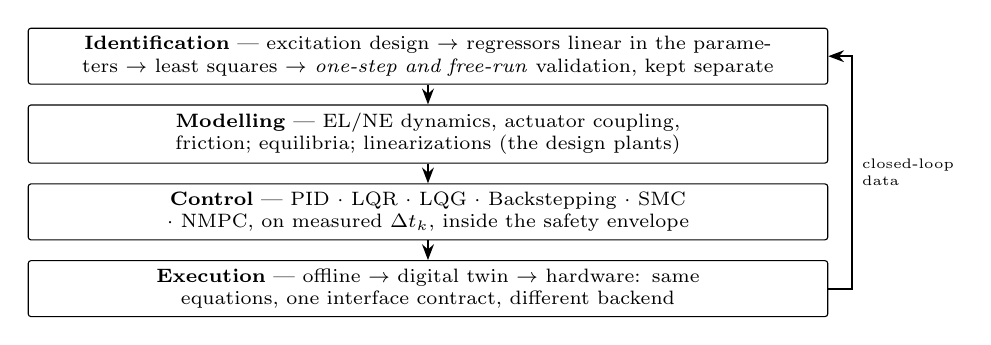
\begin{tikzpicture}[
  node distance=2.5mm,
  blk/.style={draw, rounded corners=1pt, align=center, font=\scriptsize, inner sep=3pt, text width=0.82\columnwidth},
  arr/.style={-{Stealth[length=2mm]}, thick}
]
\node[blk] (id) {\textbf{Identification} --- excitation design $\to$ regressors linear in the parameters $\to$ least squares $\to$ \emph{one-step and free-run} validation, kept separate};
\node[blk, below=of id] (mod) {\textbf{Modelling} --- EL/NE dynamics, actuator coupling, friction; equilibria; linearizations (the design plants)};
\node[blk, below=of mod] (ctl) {\textbf{Control} --- PID $\cdot$ LQR $\cdot$ LQG $\cdot$ Backstepping $\cdot$ SMC $\cdot$ NMPC, on measured $\Delta t_k$, inside the safety envelope};
\node[blk, below=of ctl] (exe) {\textbf{Execution} --- offline $\to$ digital twin $\to$ hardware: same equations, one interface contract, different backend};
\draw[arr] (id) -- (mod);
\draw[arr] (mod) -- (ctl);
\draw[arr] (ctl) -- (exe);
\draw[arr] (exe.east) -- ++(3mm,0) |- node[font=\tiny, pos=0.25, right, align=left] {closed-loop\\ data} (id.east);
\end{tikzpicture}
\caption{The workflow every platform in this series follows: identification feeds modelling, modelling feeds the controller suite, and all stages run unchanged across the three execution targets; closed-loop records return to identification.}
\label{fig:workflow}
\end{figure}
The methodology is grey-box first, black-box as cross-check, with the two validation criteria kept distinct: \emph{one-step-ahead prediction} (regression residuals with measured regressors) and \emph{free-run simulation} (model evolves on its own outputs). Local predictive quality does not imply long-horizon fidelity; both numbers are always reported.

\subsection{Linearity in the parameters}
Equations \eqref{eq:nl1}--\eqref{eq:nl2} are linear in
$\pi = [\,J_a,\ I_p,\ h,\ \kappa_g,\ \bar b_r,\ b_p\,]^{\!\top}$ with $\kappa_g = m_p g l_p$:
\begin{equation}
Y(q,\dot q,\ddot q)\,\pi = \begin{bmatrix} k_v v\\ 0\end{bmatrix},
\label{eq:regressor}
\end{equation}
where the regressor rows follow directly from \eqref{eq:nl1}--\eqref{eq:nl2}, e.g., row 1 is
$[\ \ddot\theta,\ \sin^2\!\alpha\,\ddot\theta + \sin(2\alpha)\dot\theta\dot\alpha,\ \cos\alpha\,\ddot\alpha - \sin\alpha\,\dot\alpha^2,\ 0,\ \dot\theta,\ 0\ ]$.
Accelerations are reconstructed by the filtered differentiator \eqref{eq:filtder} applied twice, and the least-squares estimate over $N$ samples is
\begin{equation}
\hat\pi = \bigl(\textstyle\sum_k Y_k^{\!\top}Y_k\bigr)^{-1}\sum_k Y_k^{\!\top}\beta_k ,
\end{equation}
with condition number of the information matrix reported as the excitation-quality metric.

\subsection{Staged experiments}
\begin{enumerate}[label=E\arabic*)]
\item \emph{Pendulum free decay (hanging).} Release from a small angle with the arm locked: \eqref{eq:hanging} gives
$\omega_d$ and the logarithmic decrement $\delta = \ln(a_j/a_{j+1})$, hence
$\zeta = \delta/\sqrt{4\pi^2+\delta^2}$, $\omega_n = \omega_d/\sqrt{1-\zeta^2}$, so
$\kappa_g/I_p = \omega_n^2$ and $b_p/I_p = 2\zeta\omega_n$. With $m_p, l_p$ from the manual, $I_p$ and $b_p$ follow.
\item \emph{Arm-only response (pendulum removed or hanging).} From \eqref{eq:lin1} with $\alpha$ quiescent, the arm is first order in velocity: $\dot\theta(s)/v(s) = k_v/(J_a s + \bar b_r)$. A step and a chirp identify the gain $k_v/\bar b_r$ and the pole $\bar b_r/J_a$; a current measurement separates $b_r$ from $k_tk_m/R_m$.
\item \emph{Coupled excitation.} PRBS or multisine voltage about zero mean (hanging configuration) excites both axes; full regressor \eqref{eq:regressor} refines $h$ and cross-terms. The first seconds of each record are discarded and signals demeaned before regression.
\item \emph{Black-box cross-check.} Discrete ARX structures $A(z^{-1})y_k = B(z^{-1})v_k + c$ fitted by least squares on the same records; agreement of the dominant discrete poles with $e^{A T_s}$ eigenvalues validates the grey-box result.
\end{enumerate}

\subsection{Validation protocol}
Fits are reported as $\mathrm{fit} = 100\,(1 - \|y-\hat y\|/\|y-\bar y\|)$ separately for one-step and free-run on \emph{held-out} records. For the upright regime, closed-loop identification is unavoidable (the plant is unstable); the direct method on \eqref{eq:regressor} remains consistent because the regression is in the physical coordinates with measured input.

%====================================================================
\section{Control Suite}\label{sec:control}
All controllers act on \eqref{eq:voltage_model} (or its linearization \eqref{eq:AB}), command $|v|\le 5$~V in the balance regime, use rate estimates from \eqref{eq:filtder} or the tachometer, and advance internal states with the measured $\Delta t_k$ per \eqref{eq:measured_dt}.

\subsection{Energy-based swing-up with mode switching}\label{sec:swing}
From \eqref{eq:Edot}, choosing the arm acceleration
\begin{equation}
u_{\mathrm{acc}} = \sat_{a_{\max}}\!\bigl(k_E\,(E - E_r)\,\sign(\dot\alpha\cos\alpha)\bigr),\qquad E_r = 0,
\label{eq:swingup}
\end{equation}
renders $\dot E = -h\cos\alpha\,\dot\alpha\,u_{\mathrm{acc}} - b_p\dot\alpha^2$ sign-definite toward $E_r$ away from $\dot\alpha\cos\alpha=0$: the pendulum energy is pumped monotonically toward the upright homoclinic level. The Lyapunov-like function $W = \tfrac12(E-E_r)^2$ satisfies $\dot W \le -k_E\,h\,|\cos\alpha\,\dot\alpha|\,(E-E_r)^2 + b_p\dot\alpha^2|E-E_r|$, giving convergence to a neighbourhood of $E_r$ dominated by pivot friction. The acceleration command is realized in voltage through the arm dynamics \eqref{eq:lin1} and motor model \eqref{eq:motor_static}:
\begin{equation}
v = \frac{1}{k_v}\Bigl(J_a\,u_{\mathrm{acc}} + \bar b_r\,\dot\theta\Bigr),
\end{equation}
saturated at $V_{\max}$. \textbf{Mode logic (implemented):} balance authority engages iff $|\alpha| \le \alpha_c = 10^\circ$; outside the capture zone the balance command is zero and \eqref{eq:swingup} (or manual swing in the hardware baseline captures) is active. Hysteresis on $\alpha_c$ and a rate condition $|\dot\alpha|\le\dot\alpha_c$ prevent chattering between modes at the boundary.

\subsection{PID and the implemented balance law}
The scalar PID in filtered-derivative form on an error $e$:
\begin{equation}
v = k_p e + k_i \int_0^t e\,d\sigma + k_d\,\hat{\dot e},\qquad
\hat{\dot e}\ \text{from \eqref{eq:filtder}},
\end{equation}
with conditional anti-windup (integration halted while $|v|$ saturates). For the pendulum, single-loop PID on $\alpha$ alone cannot stabilize the upright equilibrium with arm regulation (the arm coordinate is not detectable from $\alpha$); the practical structure is the \emph{two-angle PD} --- equivalently full state feedback:
\begin{equation}
\boxed{\;v = -K\,(x_r - x),\qquad
K = [-1.2247,\ 24.9044,\ -0.6877,\ 3.1321],\;}
\label{eq:balanceK}
\end{equation}
with $x_r = [\theta_r,0,0,0]^{\!\top}$, $|v|\le5$~V, active in the capture zone --- this is the exact law our hardware campaign runs at 500~Hz (0 amplifier faults across all trials). Its terms read as PD on the arm ($k_{p\theta} = 1.2247$, $k_{d\theta}=0.6877$ effective) plus stabilizing PD on the pendulum ($k_{p\alpha}=24.9044$, $k_{d\alpha}=3.1321$), the pendulum loop dominating as the instability requires.

\subsection{LQR}
For $\dot x = Ax + Bv$ of \eqref{eq:AB}, minimize
$J = \int_0^\infty (x^{\!\top}Qx + r v^2)\,dt$, $Q = Q^{\!\top}\!\succeq0$, $r>0$. The optimal law is $v = -K_{\mathrm{lqr}}x$ with
\begin{equation}
K_{\mathrm{lqr}} = r^{-1}B^{\!\top}P,\qquad
A^{\!\top}P + PA - r^{-1}PBB^{\!\top}P + Q = 0,
\label{eq:care}
\end{equation}
$P\succ0$ the stabilizing CARE solution. Weight selection follows Bryson scaling $Q = \diag(1/\theta_{\max}^2,\,1/\alpha_{\max}^2,\,\ldots)$, $r = 1/V_{\max}^2$, then iterating on the closed-loop poles against the delay margin $\tau_d$. The implemented gain \eqref{eq:balanceK} is of this family (state-feedback synthesis on the upright linearization); reference tracking uses $x_r$ as in \eqref{eq:balanceK} with zero feedforward because the equilibrium input is zero.

\subsection{LQG}
With encoder-only output $y = Cx + n$ and process disturbance $w$, the Kalman--Bucy estimator
\begin{equation}
\dot{\hat x} = A\hat x + Bv + L\,(y - C\hat x),\quad
L = \Sigma C^{\!\top} R_n^{-1},
\end{equation}
with $\Sigma$ the stabilizing solution of the filter CARE
$A\Sigma + \Sigma A^{\!\top} - \Sigma C^{\!\top}R_n^{-1}C\Sigma + Q_w = 0$,
feeds the LQR gain, $v = -K_{\mathrm{lqr}}\hat x + K_{\mathrm{lqr}}x_r$. Separation holds for the nominal linear plant; in implementation the estimator is advanced by explicit Euler with the measured $\Delta t_k$, and $R_n$ is set from the encoder quantization variance $q_\theta^2/12$ while $Q_w$ absorbs friction-model error. LQG's known fragility (no guaranteed margins) is the standard motivation for verifying the loop against the identified uncertainty of Section~\ref{sec:id}.

\subsection{Backstepping via collocated partial feedback linearization}\label{sec:bs}
Underactuation forbids full feedback linearization, but the \emph{collocated} PFL is exact: treat the arm acceleration as a virtual input $\nu = \ddot\theta$. From \eqref{eq:nl2},
\begin{equation}
I_p\ddot\alpha = m_p g l_p\sin\alpha - b_p\dot\alpha + \tfrac12 I_p\sin(2\alpha)\dot\theta^2 - h\cos\alpha\,\nu ,
\label{eq:pfl}
\end{equation}
a second-order pendulum subsystem driven by $\nu$ through the invertible gain $-h\cos\alpha$ (nonzero for $|\alpha|<\pi/2$). Backstepping on \eqref{eq:pfl}: with $z_1 = \alpha$, choose the stabilizing virtual rate $\dot\alpha_d = -c_1 z_1$ and let $z_2 = \dot\alpha + c_1\alpha$. Then
\begin{equation}
V_{\mathrm{bs}} = \tfrac12 z_1^2 + \tfrac12 z_2^2,\qquad
\dot V_{\mathrm{bs}} = z_1\dot z_1 + z_2\dot z_2 ,
\end{equation}
and selecting $\nu$ so that $\ddot\alpha = -c_1\dot\alpha - z_1 - c_2 z_2$, i.e.
\begin{multline}
\nu = \frac{1}{h\cos\alpha}\Bigl(m_p g l_p\sin\alpha - b_p\dot\alpha + \tfrac{I_p}{2}\sin(2\alpha)\dot\theta^2 \\
+ I_p\bigl(c_1\dot\alpha + z_1 + c_2 z_2\bigr)\Bigr),
\end{multline}
gives $\dot V_{\mathrm{bs}} = -c_1 z_1^2 - c_2 z_2^2 \le 0$ on the pendulum subsystem; arm regulation is recovered by augmenting $\nu \mathrel{+}= -c_3(\theta-\theta_r) - c_4\dot\theta$ inside the pendulum's stability margin (the standard inner--outer arrangement for Furuta-class plants). The physical torque then follows from the arm equation \eqref{eq:nl1} (inverse dynamics) and \eqref{eq:motor_static} maps it to voltage.

\subsection{Sliding-mode control}
Define the coupled sliding surface
\begin{equation}
s = \lambda_\alpha\,\alpha + \dot\alpha + \lambda_\theta(\theta-\theta_r) + \lambda_{\dot\theta}\dot\theta ,
\end{equation}
with the weights chosen so that $s=0$ restricted to the linearized dynamics \eqref{eq:AB} is Hurwitz (a one-dimensional constraint on a controllable pair). The control is equivalent-plus-switching,
\begin{equation}
v = v_{\mathrm{eq}} - \frac{\eta}{k_s}\,\sat\!\Bigl(\frac{s}{\phi}\Bigr),\qquad
v_{\mathrm{eq}}:\ \dot s\big|_{v_{\mathrm{eq}}} = 0,
\end{equation}
where $k_s = \partial \dot s/\partial v > 0$ from \eqref{eq:AB} and $\sat(\cdot)$ is the boundary-layer saturation replacing $\sign(\cdot)$ to suppress chattering (an explicit trade of asymptotic accuracy $|s|\le\phi$ for actuator health). Reaching is certified by $V_s = \tfrac12 s^2$: outside the layer, $\dot V_s = s\dot s \le -\eta|s| + |s|\,\bar\rho$, negative definite provided $\eta > \bar\rho$, the bound on matched model error --- the identified uncertainty of Section~\ref{sec:id} supplies $\bar\rho$, making the robustness claim quantitative rather than rhetorical.

\subsection{Nonlinear model predictive control}
At each step solve, over the prediction horizon $N$,
\begin{align}
\min_{u_0,\dots,u_{N-1}}\ &\sum_{k=0}^{N-1}\Bigl(\tilde x_k^{\!\top}Q\tilde x_k + r u_k^2\Bigr) + \tilde x_N^{\!\top}P_f\tilde x_N \nonumber\\
\text{s.t.}\quad & x_{k+1} = f_d(x_k, u_k) \ \ \text{(RK4 of \eqref{eq:voltage_model}, step } \Delta t_p),\nonumber\\
& |u_k| \le 5\,\mathrm{V},\qquad |\theta_k|\le\theta_{\max},
\label{eq:nmpc}
\end{align}
with $\tilde x = x - x_r$, terminal weight $P_f$ from the CARE \eqref{eq:care} (so the terminal cost is a local CLF), and apply only $u_0$ (receding horizon). Nominal stability follows from the standard terminal-cost argument: $V_N(x) = $ optimal cost is a Lyapunov function when $P_f$ and the terminal region are consistent with the LQR law. Real-time feasibility at the 500~Hz class is obtained by the same reductions we validated on the Aero2 campaign: short horizons ($N\!\sim\!5$--10), move blocking (constant $u$ over the horizon), warm-starting from the shifted previous solution, and, in the extreme, restriction of the search to a small candidate grid centred on the inverse-dynamics command --- each reduction is a documented approximation of \eqref{eq:nmpc}, not a new controller.

%====================================================================
\section{Execution Modes and the Digital Twin}
The same equations serve three targets. \emph{Offline}: \eqref{eq:voltage_model} integrated by RK4, with the sensor physics of Section~\ref{sec:sensors} (quantization \eqref{eq:quant}, filtered rates, ZOH input, measured-$\Delta t$ jitter model) injectable so that controller tuning transfers. \emph{Digital twin}: the QLabs virtual QUBE exposes the identical interface contract (angles, rates, voltage command) over the vendor API; correspondence is checked by replaying identical excitations and comparing one-step and free-run fits. \emph{Hardware}: the physical device through the vendor Python interface at 500~Hz with the safety envelope of Section~\ref{sec:safety}. The controller equations of Section~\ref{sec:control} are common to all three; only the backend changes --- the architectural discipline that makes twin-validated tuning meaningful on hardware.

%====================================================================
\section{Conclusion}
The QUBE-Servo~3 was developed as a complete physical system: energy source, PWM amplifier, DC-motor electromechanics with back-EMF damping, mechanism and friction physics, encoder quantization and rate estimation, USB-loop timing with the measured-$\Delta t$ rule, and the safety envelope --- followed by the Euler--Lagrange/Newton--Euler dynamics, the two operating regimes (nonlinear swing-up model and upright balance linearization, including the hanging model used for safe identification), a grey-box identification methodology linear in the physical parameters with one-step/free-run validation kept distinct, and the full controller suite: energy swing-up with capture logic, the implemented state-feedback balance law \eqref{eq:balanceK}, LQR/LQG, backstepping via collocated PFL, boundary-layer SMC with a quantitative reaching condition, and NMPC with its documented real-time reductions. This is the mathematical basis on which the offline, digital-twin, and hardware implementations of this platform are built and validated.

\vspace{6pt}
\noindent\textit{Scope note.} Neuromorphic residual augmentation on this platform is deliberately excluded here; it is the subject of a companion paper.

\bibliographystyle{IEEEtran}
\begin{thebibliography}{9}
\bibitem{astrom2000} K.~J. \AA str\"om and K.~Furuta, ``Swinging up a pendulum by energy control,'' \emph{Automatica}, vol.~36, no.~2, pp. 287--295, 2000.
\bibitem{cazzolato2011} B.~S. Cazzolato and Z.~Prime, ``On the dynamics of the Furuta pendulum,'' \emph{J. Control Sci. Eng.}, 2011.
\bibitem{quanser_qube3} Quanser Consulting Inc., \emph{QUBE-Servo 3 User Manual}, Markham, ON, Canada.
\bibitem{khalil2002} H.~K. Khalil, \emph{Nonlinear Systems}, 3rd ed. Prentice Hall, 2002.
\bibitem{franklin2015} G.~F. Franklin, J.~D. Powell, and A.~Emami-Naeini, \emph{Feedback Control of Dynamic Systems}, 7th ed. Pearson, 2015.
\bibitem{franklin1998} G.~F. Franklin, J.~D. Powell, and M.~Workman, \emph{Digital Control of Dynamic Systems}, 3rd ed. Addison-Wesley, 1998.
\bibitem{utkin1992} V.~Utkin, \emph{Sliding Modes in Control and Optimization}. Springer, 1992.
\bibitem{krstic1995} M.~Krsti\'c, I.~Kanellakopoulos, and P.~Kokotovi\'c, \emph{Nonlinear and Adaptive Control Design}. Wiley, 1995.
\bibitem{rawlings2017} J.~B. Rawlings, D.~Q. Mayne, and M.~Diehl, \emph{Model Predictive Control: Theory, Computation, and Design}, 2nd ed. Nob Hill, 2017.
\end{thebibliography}

\end{document}
